In the last section, we have developed a formal language for representing multigrid methods with the use of simple state transition functions.
Furthermore, we have shown how it is possible to formulate a context-free grammar for generating representations of arbitrarily-structured multigrid methods in that language.
As we have already discussed in this section, due to the context-independence of each production of this grammar, each of its derivations can be formulated as a tree.
For this purpose, consider again the three-grid method shown in Algorithm~\ref{alg:example-three-grid-method}.
We can now express this method as a sequence of the productions defined in Section~\ref{sec:multigrid-grammar}, which leads to the derivation tree shown in Figure~\ref{fig:example-three-grid-method-derivation-tree}.
\begin{figure}
	\centering
	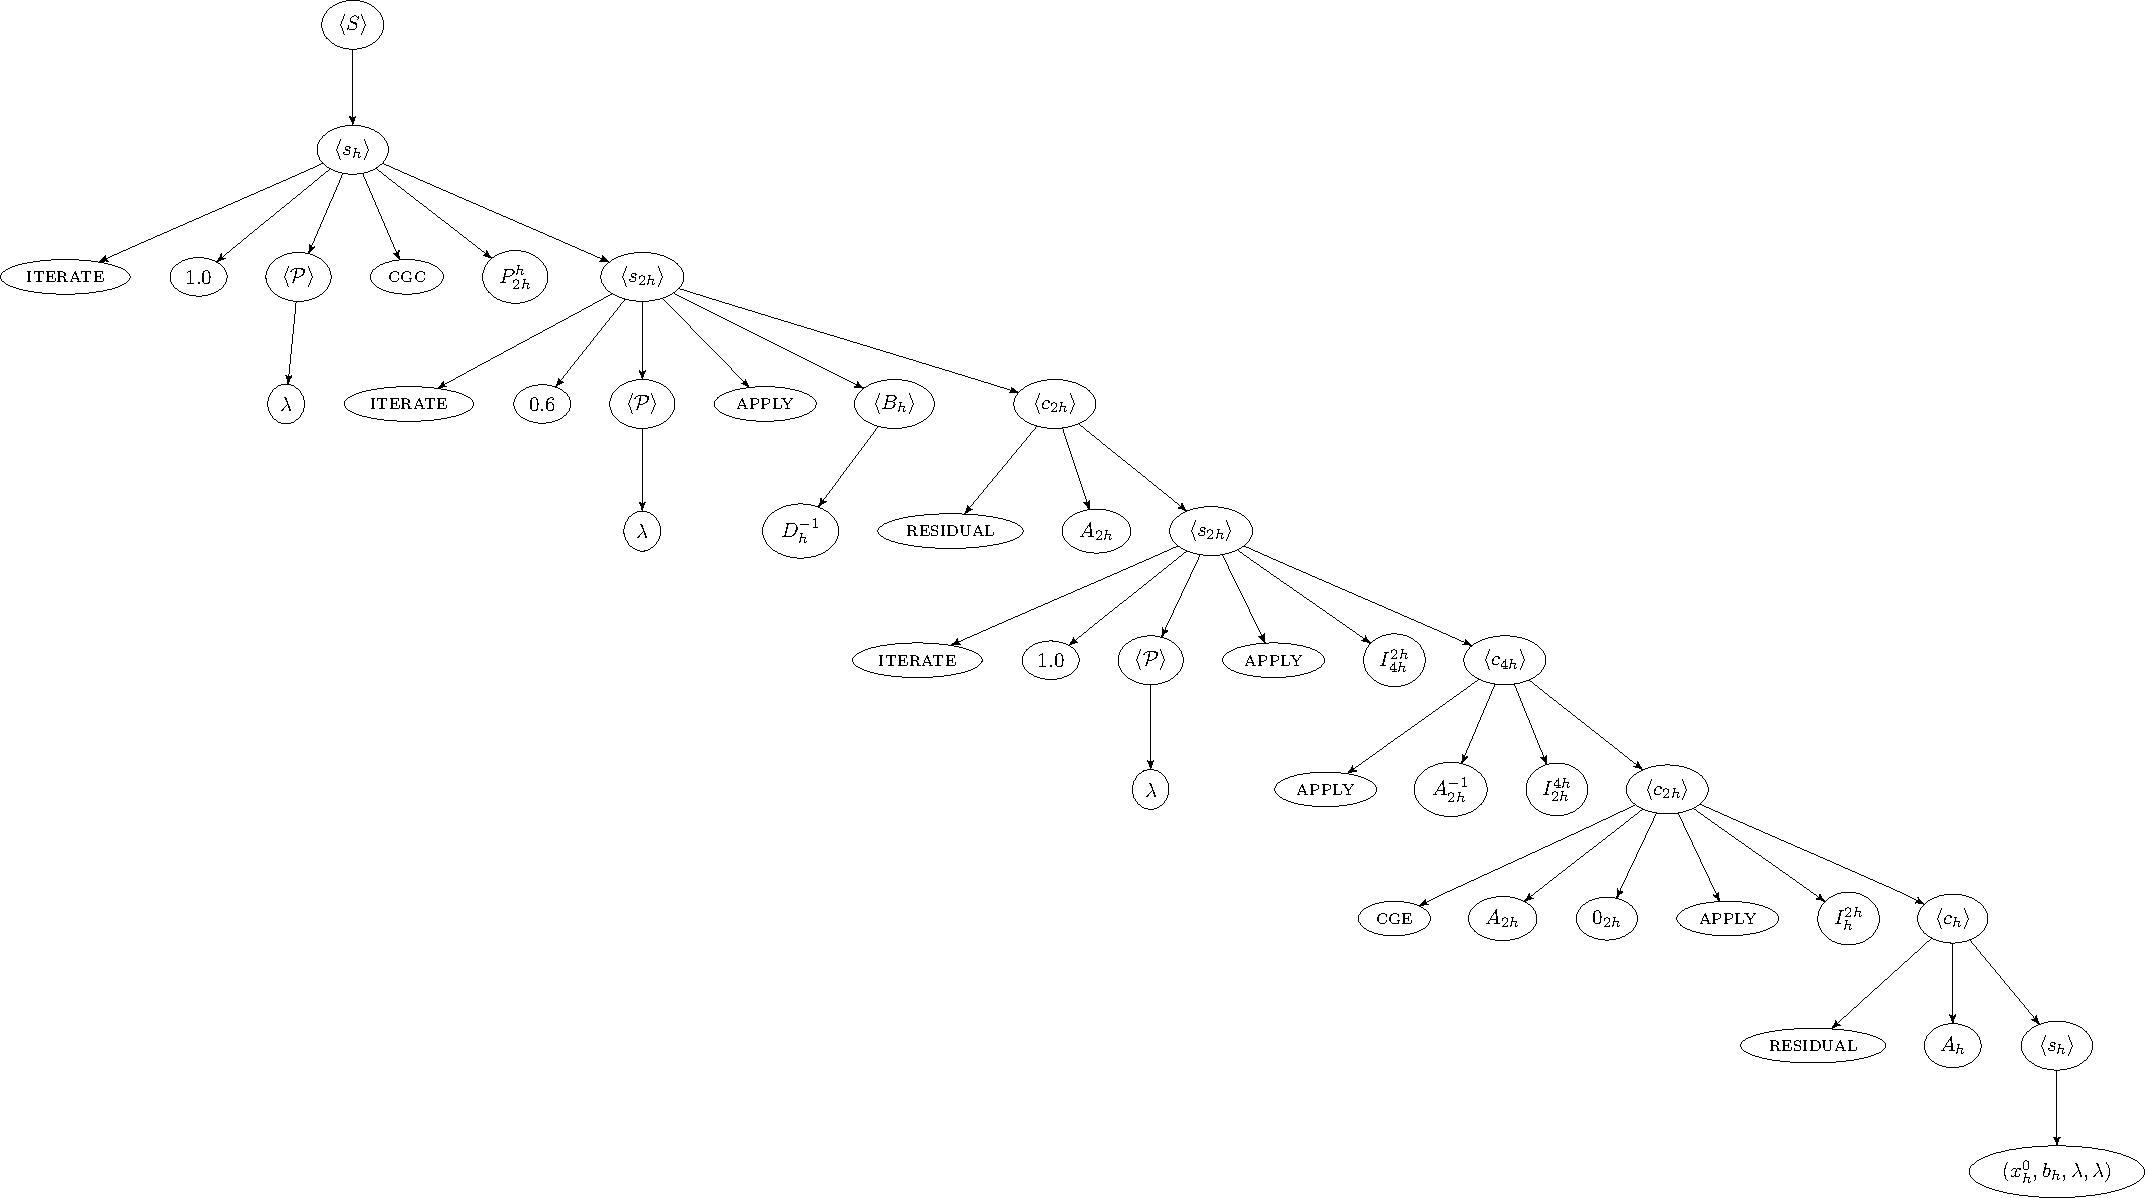
\includegraphics[width=\textwidth]{figures/trees/three_grid_method_grammar_tree.pdf}
	\caption{Grammar derivation tree for the three-grid method shown in Algorithm~\ref{alg:example-three-grid-method}.}
	\label{fig:example-three-grid-method-derivation-tree}
\end{figure}   

\begin{figure}
	\centering
	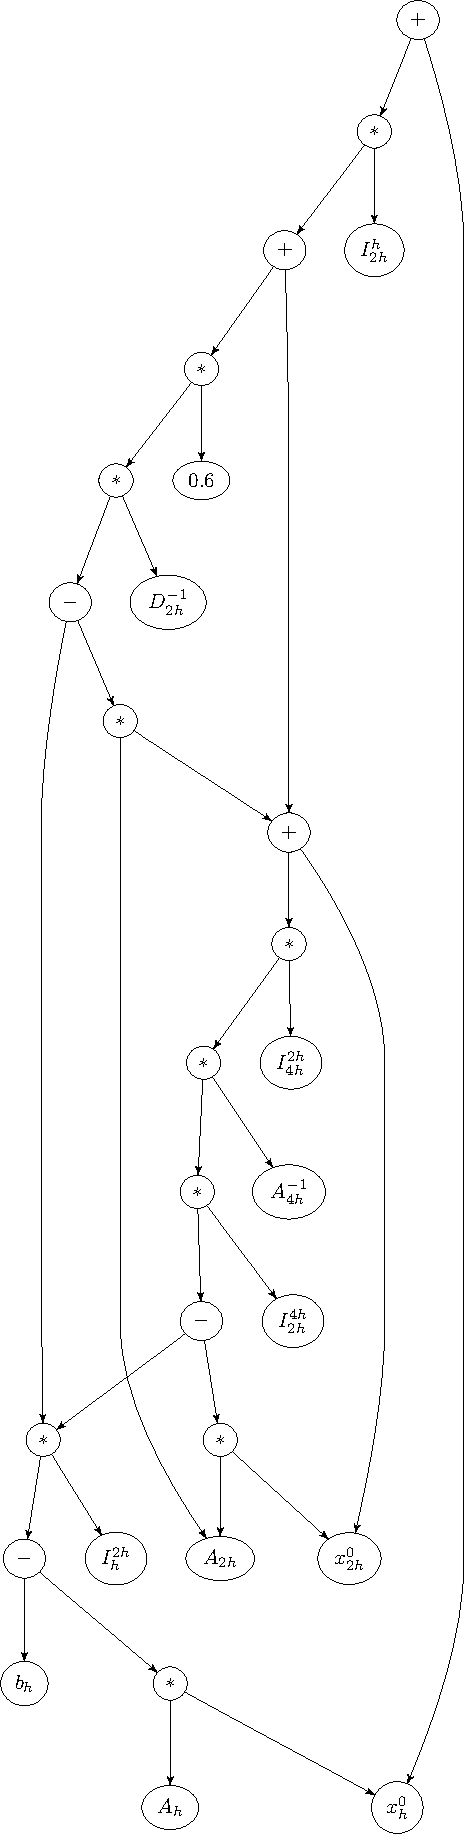
\includegraphics[height=\textheight]{figures/trees/three_grid_method_computational_graph.pdf}
	\caption{Computational graph for the three-grid method shown in Algorithm~\ref{alg:example-three-grid-method}.}
	\label{fig:example-three-grid-method-computational graph}
\end{figure}  